
\documentclass[10pt]{article}

\usepackage[a4paper,margin=0.65in]{geometry}
\usepackage{amsmath,amssymb}
\usepackage{graphicx}
\usepackage{booktabs}
\usepackage{array}
\usepackage{float}
\usepackage{hyperref}
\usepackage{enumitem}
\usepackage{xcolor}
\usepackage{tikz}
\usetikzlibrary{positioning,arrows.meta,shapes.geometric,fit,calc}

\setlist{nosep,leftmargin=*}
\renewcommand{\arraystretch}{1.2}
\setlength{\parindent}{0pt}
\setlength{\parskip}{2pt}

\tikzset{
layer/.style={
draw,
rounded corners,
minimum width=1.7cm,
minimum height=0.65cm,
align=center,
fill=blue!10,
font=\scriptsize
},
smalllayer/.style={
draw,
rounded corners,
minimum width=1.35cm,
minimum height=0.58cm,
align=center,
fill=green!10,
font=\scriptsize
},
arrow/.style={
-{Latex[length=2mm]},
thin
}
}

\begin{document}

%%%%%%%%%%%%%%%%%%%%%%%%%%%%%%%%%%%%%%%%%%%%%%%%%%%%%%%%%%%%
% TITLE
%%%%%%%%%%%%%%%%%%%%%%%%%%%%%%%%%%%%%%%%%%%%%%%%%%%%%%%%%%%%

\begin{center}

{\large\textbf{Shiv Nadar University Chennai}}

\vspace{2mm}

{\normalsize\textbf{CS3807 -- Deep Learning Laboratory}}

\vspace{2mm}

{\large\textbf{Experiment 6}}

\vspace{1mm}

{\normalsize\textbf{End-to-End Study of RNN, LSTM and GRU for}}

{\normalsize\textbf{Sequence Learning and Video Understanding}}

\end{center}

\vspace{3mm}

\begin{tabular}{|p{3.4cm}|p{9.0cm}|p{1.4cm}|}
\hline
Degree \& Branch &
B.Tech Artificial Intelligence \& Data Science &
Semester V\\
\hline
Subject Code \& Name &
CS3807 -- Deep Learning Laboratory &
AY: 2026--27\\
\hline
\end{tabular}

%%%%%%%%%%%%%%%%%%%%%%%%%%%%%%%%%%%%%%%%%%%%%%%%%%%%%%%%%%%%
\section*{1. Objective}

The objective of this experiment is to develop an end-to-end understanding of
recurrent sequence learning by implementing and comparing Vanilla RNN, LSTM
and GRU models. The experiment also introduces Backpropagation Through Time
(BPTT), the limitations of conventional RNNs, and the use of CNN-extracted
features with recurrent networks for video understanding.

The experiment uses the UCI Human Activity Recognition Using Smartphones
dataset as the primary sequence dataset. Students will prepare temporal input
sequences, visualize them, train RNN/LSTM/GRU models, compare their
performance, analyze convergence and generalization, and extend the pipeline
to video understanding using CNN feature extraction followed by an LSTM or
GRU.

A small synthetic sequence-to-sequence task is included at the end to
demonstrate the encoder--decoder framework.

%%%%%%%%%%%%%%%%%%%%%%%%%%%%%%%%%%%%%%%%%%%%%%%%%%%%%%%%%%%%
\section*{2. Learning Outcomes}

After completing this experiment, students will be able to:

\begin{itemize}
\item represent sequential data using the $(N,T,F)$ input format;
\item explain the architecture and operation of a Vanilla RNN;
\item explain Backpropagation Through Time and the vanishing/exploding gradient challenges;
\item implement sequence classification using SimpleRNN, LSTM and GRU;
\item compare RNN, LSTM and GRU using quantitative performance measures;
\item interpret training/validation curves and confusion matrices;
\item explain the role of CNNs in extracting spatial features from video frames;
\item construct a CNN--LSTM or CNN--GRU pipeline for video understanding;
\item explain the encoder--decoder architecture for sequence-to-sequence learning; and
\item draw conclusions using predictive performance, model complexity and computational cost.
\end{itemize}

%%%%%%%%%%%%%%%%%%%%%%%%%%%%%%%%%%%%%%%%%%%%%%%%%%%%%%%%%%%%
\section*{3. Dataset and Experimental Setup}

\textbf{Primary Dataset: UCI Human Activity Recognition Using Smartphones}

The UCI Human Activity Recognition (HAR) dataset contains smartphone sensor
measurements collected from subjects performing six activities:

\begin{itemize}
\item WALKING
\item WALKING\_UPSTAIRS
\item WALKING\_DOWNSTAIRS
\item SITTING
\item STANDING
\item LAYING
\end{itemize}

The experiment should use the raw inertial signal files rather than only the
already-computed 561-feature vectors. Each activity window contains 128
temporal measurements. The three-axis body acceleration, three-axis
gyroscope and three-axis total acceleration signals provide nine channels.

Thus, the desired input representation is

\[
X\in\mathbb{R}^{N\times128\times9}.
\]

The dataset can be obtained from:

\url{https://archive.ics.uci.edu/dataset/240/human+activity+recognition+using+smartphones}

\textbf{Recommended laboratory subset:} To keep execution time small, use
the first 1500--3000 training windows while preserving all six classes and
approximately balanced class representation. For a complete study, the full
training and test partitions may be used.

\textbf{Important:} The same train/validation/test protocol and preprocessing
must be used for RNN, LSTM and GRU so that the comparison is controlled.

\subsection*{Expected Input}

For one sample:

\[
X_i\in\mathbb{R}^{128\times9}.
\]

For a batch of 32 samples:

\[
X_{\mathrm{batch}}\in\mathbb{R}^{32\times128\times9}.
\]

The dimensions represent:

\begin{center}
\begin{tabular}{|c|c|l|}
\hline
Dimension & Meaning & Example\\
\hline
$N$ & Number of sequences & 1500\\
$T$ & Time steps per sequence & 128\\
$F$ & Features/channels per time step & 9\\
\hline
\end{tabular}
\end{center}

Therefore, the model must receive a three-dimensional tensor rather than a
conventional two-dimensional tabular matrix.

%%%%%%%%%%%%%%%%%%%%%%%%%%%%%%%%%%%%%%%%%%%%%%%%%%%%%%%%%%%%
\section*{4. Overall Experimental Pipeline}

The complete sequence-classification pipeline is:

\begin{center}
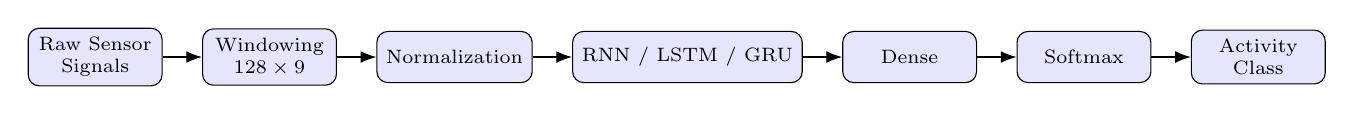
\begin{tikzpicture}[node distance=5mm]
\node[layer](a){Raw Sensor\\Signals};
\node[layer,right=of a](b){Windowing\\$128\times9$};
\node[layer,right=of b](c){Normalization};
\node[layer,right=of c](d){RNN / LSTM / GRU};
\node[layer,right=of d](e){Dense};
\node[layer,right=of e](f){Softmax};
\node[layer,right=of f](g){Activity\\Class};

\foreach \x/\y in {a/b,b/c,c/d,d/e,e/f,f/g}
\draw[arrow](\x)--(\y);
\end{tikzpicture}
\end{center}

The three recurrent models must use the same input, output layer, optimizer,
batch size and evaluation protocol.

%%%%%%%%%%%%%%%%%%%%%%%%%%%%%%%%%%%%%%%%%%%%%%%%%%%%%%%%%%%%
\section*{5. Preprocessing}

Perform the following preprocessing steps:

\begin{enumerate}
\item Load the raw inertial signals.
\item Arrange every observation window as $128\times9$.
\item Assign one activity label to each window.
\item Encode the six activity labels.
\item Normalize the input using statistics calculated from the training data.
\item Create training, validation and test sets.
\item Verify the class distribution.
\end{enumerate}

\textbf{Suggested split:}

\[
70\% \text{ training},\qquad
15\% \text{ validation},\qquad
15\% \text{ testing}.
\]

The test data must not be used during model selection or hyperparameter tuning.

\subsection*{Expected Preprocessing Output}

Students must print:

\begin{verbatim}
Input tensor shape:
Training   : (N_train, 128, 9)
Validation : (N_val,   128, 9)
Testing    : (N_test,  128, 9)

Number of classes: 6
Number of features per time step: 9
Sequence length: 128
\end{verbatim}

The actual values of $N_{\mathrm{train}}$, $N_{\mathrm{val}}$ and
$N_{\mathrm{test}}$ depend on the selected subset.

%%%%%%%%%%%%%%%%%%%%%%%%%%%%%%%%%%%%%%%%%%%%%%%%%%%%%%%%%%%%
\section*{6. Temporal Data Visualization}

Select representative sequences from at least three different activity
classes.

\textbf{Plot 1: Sensor signal versus time}

\begin{itemize}
\item X-axis: Time step (1--128)
\item Y-axis: Sensor value
\item Plot at least three representative channels.
\item Include examples from different activity classes.
\end{itemize}

Students should observe that temporal patterns differ across activities.

\textbf{Required inference:}

\begin{enumerate}
\item What temporal pattern is visible?
\item Which activities exhibit similar patterns?
\item Why is the ordering of measurements important?
\end{enumerate}

%%%%%%%%%%%%%%%%%%%%%%%%%%%%%%%%%%%%%%%%%%%%%%%%%%%%%%%%%%%%
\section*{7. Vanilla RNN Architecture}

A Vanilla RNN maintains a hidden state that is updated at every time step:

\[
h_t=\tanh(W_xx_t+W_hh_{t-1}+b_h).
\]

The output can be written as

\[
y_t=g(W_yh_t+b_y).
\]

For sequence classification, the final hidden representation can be passed
to a classifier.

\begin{center}
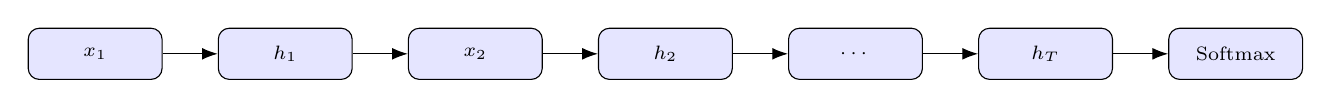
\begin{tikzpicture}[node distance=7mm]
\node[layer](x1){$x_1$};
\node[layer,right=of x1](h1){$h_1$};
\node[layer,right=of h1](x2){$x_2$};
\node[layer,right=of x2](h2){$h_2$};
\node[layer,right=of h2](x3){$\cdots$};
\node[layer,right=of x3](h3){$h_T$};
\node[layer,right=of h3](y){Softmax};

\draw[arrow](x1)--(h1);
\draw[arrow](h1)--(x2);
\draw[arrow](x2)--(h2);
\draw[arrow](h2)--(x3);
\draw[arrow](x3)--(h3);
\draw[arrow](h3)--(y);
\end{tikzpicture}
\end{center}

The diagram represents the unrolled view of an RNN. The same recurrent weights
are reused across time steps.

%%%%%%%%%%%%%%%%%%%%%%%%%%%%%%%%%%%%%%%%%%%%%%%%%%%%%%%%%%%%
\section*{8. Backpropagation Through Time}

When an RNN is unrolled, the loss depends on the sequence of hidden states.
Backpropagation Through Time (BPTT) propagates the error backward through
the recurrent steps.

\begin{center}
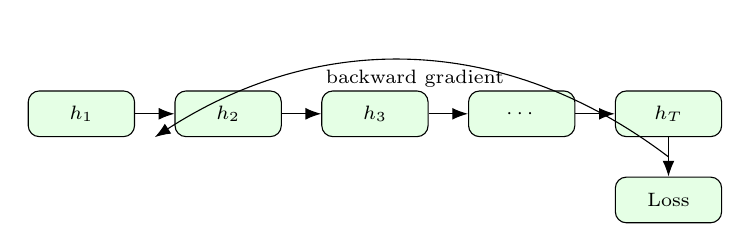
\begin{tikzpicture}[node distance=5mm]
\node[smalllayer](a){$h_1$};
\node[smalllayer,right=of a](b){$h_2$};
\node[smalllayer,right=of b](c){$h_3$};
\node[smalllayer,right=of c](d){$\cdots$};
\node[smalllayer,right=of d](e){$h_T$};
\node[smalllayer,below=of e](l){Loss};

\draw[arrow](a)--(b);
\draw[arrow](b)--(c);
\draw[arrow](c)--(d);
\draw[arrow](d)--(e);
\draw[arrow](e)--(l);

\draw[arrow]($(e.south)!0.5!(l.north)$) to[bend right=35]
node[below,font=\scriptsize]{backward gradient} ($(a.south)!0.5!(b.south)$);
\end{tikzpicture}
\end{center}

Students should explain that repeated multiplication of derivatives through
many time steps can cause gradients to become extremely small or extremely
large.

\subsection*{Challenges}

\begin{itemize}
\item Vanishing gradients
\item Exploding gradients
\item Difficulty learning long-term dependencies
\item Sequential computation and limited parallelism
\end{itemize}

The vanishing-gradient problem can be conceptually represented as

\[
\left|\frac{\partial h_t}{\partial h_{t-k}}\right|\rightarrow0
\]

while exploding gradients correspond to very large gradient magnitudes.

\subsection*{Numerical Exercise}

Consider

\[
x_1=0.5,\qquad x_2=0.7,\qquad x_3=0.2,
\]

\[
h_0=0,\qquad W_x=0.5,\qquad W_h=0.8,\qquad b=0.1.
\]

Using

\[
h_t=\tanh(W_xx_t+W_hh_{t-1}+b),
\]

calculate $h_1$, $h_2$ and $h_3$ manually.

Students must compare their calculated values with the values obtained from
a program.

%%%%%%%%%%%%%%%%%%%%%%%%%%%%%%%%%%%%%%%%%%%%%%%%%%%%%%%%%%%%
\section*{9. RNN Implementation}

Use a small recurrent architecture:

\begin{center}
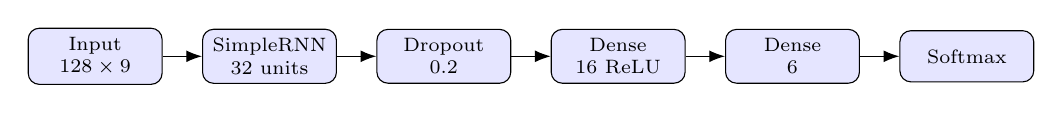
\begin{tikzpicture}[node distance=5mm]
\node[layer](a){Input\\$128\times9$};
\node[layer,right=of a](b){SimpleRNN\\32 units};
\node[layer,right=of b](c){Dropout\\0.2};
\node[layer,right=of c](d){Dense\\16 ReLU};
\node[layer,right=of d](e){Dense\\6};
\node[layer,right=of e](f){Softmax};

\foreach \x/\y in {a/b,b/c,c/d,d/e,e/f}
\draw[arrow](\x)--(\y);
\end{tikzpicture}
\end{center}

\textbf{Suggested training configuration:}

\begin{center}
\begin{tabular}{|l|l|}
\hline
Parameter & Value\\
\hline
Recurrent units & 32\\
Dropout & 0.2\\
Optimizer & Adam\\
Learning rate & $10^{-3}$\\
Batch size & 32\\
Epochs & 30\\
Loss & Sparse categorical cross-entropy\\
\hline
\end{tabular}
\end{center}

%%%%%%%%%%%%%%%%%%%%%%%%%%%%%%%%%%%%%%%%%%%%%%%%%%%%%%%%%%%%
\section*{10. LSTM Architecture}

LSTM introduces a memory cell and gates to control information flow.

The forget gate is

\[
f_t=\sigma(W_f[h_{t-1},x_t]+b_f),
\]

the input gate is

\[
i_t=\sigma(W_i[h_{t-1},x_t]+b_i),
\]

and the output gate is

\[
o_t=\sigma(W_o[h_{t-1},x_t]+b_o).
\]

The candidate cell state is

\[
\tilde{C}_t=
\tanh(W_C[h_{t-1},x_t]+b_C),
\]

and the cell state is

\[
C_t=f_tC_{t-1}+i_t\tilde{C}_t.
\]

The hidden state is

\[
h_t=o_t\tanh(C_t).
\]

\begin{center}
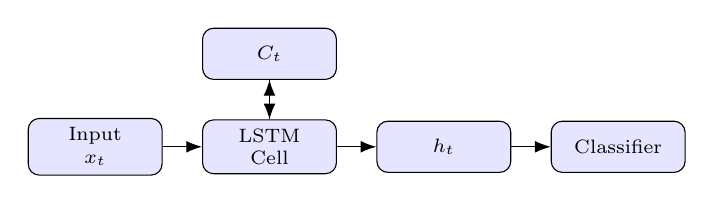
\begin{tikzpicture}[node distance=5mm]
\node[layer](a){Input\\$x_t$};
\node[layer,right=of a](b){LSTM\\Cell};
\node[layer,right=of b](c){$h_t$};
\node[layer,above=of b](d){$C_t$};
\node[layer,right=of c](e){Classifier};

\draw[arrow](a)--(b);
\draw[arrow](b)--(c);
\draw[arrow](b)--(d);
\draw[arrow](c)--(e);
\draw[arrow](d)--(b);
\end{tikzpicture}
\end{center}

\textbf{Required inference:} Explain how the cell state and gates help the
network retain or discard information over long sequences.

%%%%%%%%%%%%%%%%%%%%%%%%%%%%%%%%%%%%%%%%%%%%%%%%%%%%%%%%%%%%
\section*{11. GRU Architecture}

GRU uses two principal gates:

\[
z_t=\sigma(W_z[h_{t-1},x_t]+b_z)
\]

and

\[
r_t=\sigma(W_r[h_{t-1},x_t]+b_r).
\]

The candidate hidden state is

\[
\tilde{h}_t=
\tanh(W_h[r_t\odot h_{t-1},x_t]+b_h).
\]

The hidden state is updated using

\[
h_t=(1-z_t)h_{t-1}+z_t\tilde{h}_t.
\]

\begin{center}
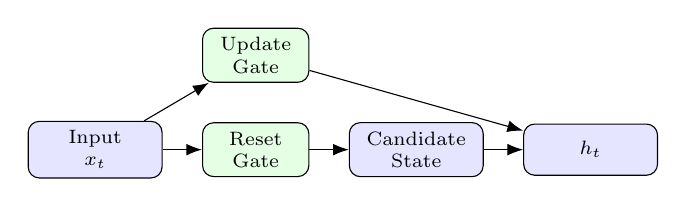
\begin{tikzpicture}[node distance=5mm]
\node[layer](a){Input\\$x_t$};
\node[smalllayer,right=of a](b){Reset\\Gate};
\node[smalllayer,above=of b](c){Update\\Gate};
\node[layer,right=of b](d){Candidate\\State};
\node[layer,right=of d](e){$h_t$};

\draw[arrow](a)--(b);
\draw[arrow](a)--(c);
\draw[arrow](b)--(d);
\draw[arrow](c)--(e);
\draw[arrow](d)--(e);
\end{tikzpicture}
\end{center}

Students should compare the number of gates and state representations in
RNN, LSTM and GRU.

%%%%%%%%%%%%%%%%%%%%%%%%%%%%%%%%%%%%%%%%%%%%%%%%%%%%%%%%%%%%
\section*{12. LSTM and GRU Implementation}

Implement the same classifier used for the RNN, replacing only the recurrent
layer.

\begin{center}
\begin{tabular}{|l|c|c|c|}
\hline
Model & Recurrent Layer & Units & Output Classes\\
\hline
RNN & SimpleRNN & 32 & 6\\
LSTM & LSTM & 32 & 6\\
GRU & GRU & 32 & 6\\
\hline
\end{tabular}
\end{center}

All other experimental conditions should remain unchanged.

%%%%%%%%%%%%%%%%%%%%%%%%%%%%%%%%%%%%%%%%%%%%%%%%%%%%%%%%%%%%
\section*{13. Required Training Plots}

For each of RNN, LSTM and GRU, generate:

\textbf{Plot 2: Training and Validation Loss}

\begin{itemize}
\item X-axis: Epoch
\item Y-axis: Loss
\item Curves: Training loss and validation loss
\end{itemize}

\textbf{Plot 3: Training and Validation Accuracy}

\begin{itemize}
\item X-axis: Epoch
\item Y-axis: Accuracy (\%)
\item Curves: Training accuracy and validation accuracy
\end{itemize}

\textbf{Inference:} Students must identify convergence, overfitting,
underfitting and the generalization gap where applicable.

%%%%%%%%%%%%%%%%%%%%%%%%%%%%%%%%%%%%%%%%%%%%%%%%%%%%%%%%%%%%
\section*{14. Performance Evaluation}

Evaluate each model on the independent test set.

The following metrics are mandatory:

\begin{itemize}
\item Accuracy
\item Precision
\item Recall
\item F1-score
\item Confusion matrix
\item Number of trainable parameters
\item Training time
\end{itemize}

For multi-class classification, report macro-averaged Precision, Recall and
F1-score.

\begin{center}
\begin{tabular}{|l|c|c|c|}
\hline
Metric & RNN & LSTM & GRU\\
\hline
Accuracy (\%) & & &\\
Macro Precision (\%) & & &\\
Macro Recall (\%) & & &\\
Macro F1 (\%) & & &\\
Parameters & & &\\
Training Time (s) & & &\\
\hline
\end{tabular}
\end{center}

%%%%%%%%%%%%%%%%%%%%%%%%%%%%%%%%%%%%%%%%%%%%%%%%%%%%%%%%%%%%
\section*{15. Confusion Matrix Analysis}

\textbf{Plot 4: Confusion Matrix}

Generate a separate confusion matrix for each model.

Students must identify:

\begin{itemize}
\item the activity with the highest recognition rate;
\item the activity with the largest number of misclassifications;
\item pairs of activities that are frequently confused; and
\item whether the errors are consistent across RNN, LSTM and GRU.
\end{itemize}

The inference must be based on the student's observed matrix rather than on
an assumed result.

%%%%%%%%%%%%%%%%%%%%%%%%%%%%%%%%%%%%%%%%%%%%%%%%%%%%%%%%%%%%
\section*{16. RNN vs. LSTM vs. GRU Comparison}

Students must complete the following table.

\begin{center}
\begin{tabular}{|l|c|c|c|}
\hline
Property & RNN & LSTM & GRU\\
\hline
Hidden state & Yes & Yes & Yes\\
Cell state & No & Yes & No\\
Forget gate & No & Yes & No\\
Input gate & No & Yes & No\\
Output gate & No & Yes & No\\
Update gate & No & No & Yes\\
Reset gate & No & No & Yes\\
Parameters & & &\\
Training time & & &\\
Test F1-score & & &\\
\hline
\end{tabular}
\end{center}

\textbf{Plot 5: Model Performance Comparison}

Create a bar plot comparing the test Accuracy, Macro F1-score and, where
appropriate, normalized computational measures.

\textbf{Required inference:}

Students should discuss the trade-off among:

\[
\text{Predictive Performance}
\quad\leftrightarrow\quad
\text{Model Complexity}
\quad\leftrightarrow\quad
\text{Training Cost}.
\]

%%%%%%%%%%%%%%%%%%%%%%%%%%%%%%%%%%%%%%%%%%%%%%%%%%%%%%%%%%%%
\section*{17. Effect of Sequence Length}

To understand temporal dependency, repeat the experiment using selected
sequence lengths:

\[
T\in\{32,64,128\}.
\]

When reducing the sequence length, truncate or construct the input consistently.

\begin{center}
\begin{tabular}{|c|c|c|c|}
\hline
Sequence Length & RNN F1 & LSTM F1 & GRU F1\\
\hline
32 & & &\\
64 & & &\\
128 & & &\\
\hline
\end{tabular}
\end{center}

\textbf{Plot 6: Sequence Length vs. Test F1-score}

Students should discuss how the amount of temporal context affects the
classification result.

%%%%%%%%%%%%%%%%%%%%%%%%%%%%%%%%%%%%%%%%%%%%%%%%%%%%%%%%%%%%
\section*{18. Video Understanding Using CNN and RNN}

This part demonstrates the application:

\[
\boxed{\text{Video Understanding using CNN + RNN}}
\]

A video is a sequence of image frames. CNNs are used to extract spatial
features from individual frames, while RNN/LSTM/GRU models the temporal
relationship among those features.

The complete pipeline is:

\begin{center}
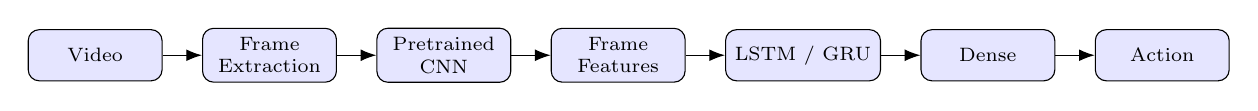
\begin{tikzpicture}[node distance=5mm]
\node[layer](a){Video};
\node[layer,right=of a](b){Frame\\Extraction};
\node[layer,right=of b](c){Pretrained\\CNN};
\node[layer,right=of c](d){Frame\\Features};
\node[layer,right=of d](e){LSTM / GRU};
\node[layer,right=of e](f){Dense};
\node[layer,right=of f](g){Action};

\foreach \x/\y in {a/b,b/c,c/d,d/e,e/f,f/g}
\draw[arrow](\x)--(\y);
\end{tikzpicture}
\end{center}

\subsection*{Recommended Dataset}

Use a small subset of the UCF101 action-recognition dataset:

\url{https://www.crcv.ucf.edu/data/UCF101.php}

Select only 3--5 action classes and a small number of videos per class so that
the experiment remains computationally manageable.

Possible classes include:

\begin{itemize}
\item Basketball
\item Biking
\item Walking
\item Running
\item TennisSwing
\end{itemize}

The objective is to understand the CNN--recurrent pipeline rather than to
train a state-of-the-art video recognition system.

%%%%%%%%%%%%%%%%%%%%%%%%%%%%%%%%%%%%%%%%%%%%%%%%%%%%%%%%%%%%
\section*{19. Expected Video Input and Output}

Sample 10 frames uniformly from each video.

Each frame is resized to

\[
224\times224\times3.
\]

A pretrained CNN such as MobileNetV2 is used only as a feature extractor.

If the CNN produces a feature vector of dimension $D$, then the recurrent
network receives:

\[
X\in\mathbb{R}^{10\times D}.
\]

For a batch of $B$ videos:

\[
X\in\mathbb{R}^{B\times10\times D}.
\]

The expected output is a probability vector over the selected action classes.

For example:

\begin{verbatim}
Predicted class : Basketball
Actual class    : Basketball
Confidence      : 0.xx
\end{verbatim}

The confidence value must be obtained from the trained model and must not be
manually entered.

%%%%%%%%%%%%%%%%%%%%%%%%%%%%%%%%%%%%%%%%%%%%%%%%%%%%%%%%%%%%
\section*{20. CNN Feature Extraction}

Use a pretrained CNN with the classification head removed.

\begin{center}
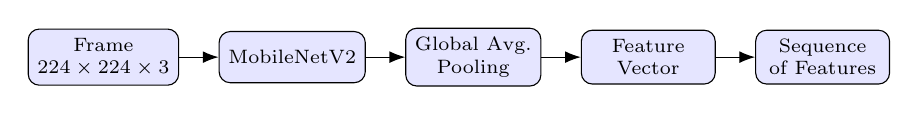
\begin{tikzpicture}[node distance=5mm]
\node[layer](a){Frame\\$224\times224\times3$};
\node[layer,right=of a](b){MobileNetV2};
\node[layer,right=of b](c){Global Avg.\\Pooling};
\node[layer,right=of c](d){Feature\\Vector};
\node[layer,right=of d](e){Sequence\\of Features};

\foreach \x/\y in {a/b,b/c,c/d,d/e}
\draw[arrow](\x)--(\y);
\end{tikzpicture}
\end{center}

Do not train the CNN from scratch. Freeze the pretrained CNN and extract
features first. Then train the recurrent classifier.

\textbf{Required observation:}

Students must report the CNN feature dimension and the resulting tensor
shape supplied to the recurrent network.

%%%%%%%%%%%%%%%%%%%%%%%%%%%%%%%%%%%%%%%%%%%%%%%%%%%%%%%%%%%%
\section*{21. CNN--LSTM / CNN--GRU Model}

Use the following architecture:

\begin{center}
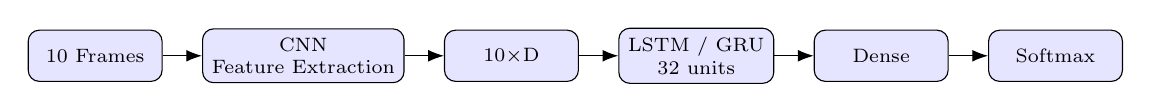
\begin{tikzpicture}[node distance=5mm]
\node[layer](a){10 Frames};
\node[layer,right=of a](b){CNN\\Feature Extraction};
\node[layer,right=of b](c){10$\times$D};
\node[layer,right=of c](d){LSTM / GRU\\32 units};
\node[layer,right=of d](e){Dense};
\node[layer,right=of e](f){Softmax};

\foreach \x/\y in {a/b,b/c,c/d,d/e,e/f}
\draw[arrow](\x)--(\y);
\end{tikzpicture}
\end{center}

\textbf{Plot 7: Video Sample Frames}

Display a representative sequence of sampled frames from one video.

Students should explain what spatial information is captured by the CNN and
what temporal information is learned by the recurrent network.

\textbf{Plot 8: Video Training and Validation Curves}

Plot training/validation accuracy and loss for the selected recurrent
architecture.

\textbf{Plot 9: Video Confusion Matrix}

Analyze class-level recognition and temporal confusions.

%%%%%%%%%%%%%%%%%%%%%%%%%%%%%%%%%%%%%%%%%%%%%%%%%%%%%%%%%%%%
\section*{22. Sequence-to-Sequence Learning}

Sequence-to-sequence learning maps one sequence to another.

For a simple laboratory task, construct a synthetic reversal dataset.

Example:

\[
[1,4,7,2]\rightarrow[2,7,4,1].
\]

Generate several thousand short sequences using integers from a fixed range.

The task is intentionally simple so that the encoder--decoder mechanism can
be studied without a large external dataset.

\begin{center}
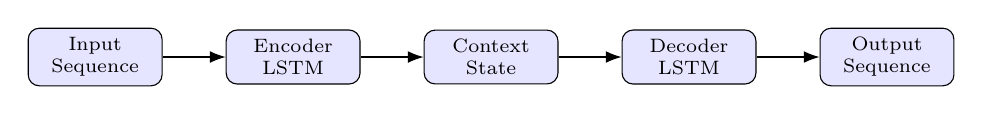
\begin{tikzpicture}[node distance=8mm]
\node[layer](a){Input\\Sequence};
\node[layer,right=of a](b){Encoder\\LSTM};
\node[layer,right=of b](c){Context\\State};
\node[layer,right=of c](d){Decoder\\LSTM};
\node[layer,right=of d](e){Output\\Sequence};

\foreach \x/\y in {a/b,b/c,c/d,d/e}
\draw[arrow](\x)--(\y);
\end{tikzpicture}
\end{center}

The encoder converts the input sequence into a learned representation.
The decoder generates the output sequence one element at a time.

%%%%%%%%%%%%%%%%%%%%%%%%%%%%%%%%%%%%%%%%%%%%%%%%%%%%%%%%%%%%
\section*{23. Expected Sequence-to-Sequence Input and Output}

\textbf{Input example:}

\[
[3,8,1,5]
\]

\textbf{Expected output:}

\[
[5,1,8,3].
\]

Students must display at least five test examples in the report.

\begin{center}
\begin{tabular}{|c|c|c|}
\hline
Sample & Input Sequence & Predicted Output\\
\hline
1 & &\\
2 & &\\
3 & &\\
4 & &\\
5 & &\\
\hline
\end{tabular}
\end{center}

%%%%%%%%%%%%%%%%%%%%%%%%%%%%%%%%%%%%%%%%%%%%%%%%%%%%%%%%%%%%
\section*{24. Sequence-to-Sequence Evaluation}

Report:

\begin{itemize}
\item Token accuracy
\item Sequence accuracy
\item Training loss
\item Validation loss
\end{itemize}

Token accuracy is

\[
\text{Token Accuracy}
=
\frac{\text{Correctly predicted tokens}}
{\text{Total tokens}}.
\]

Sequence accuracy is

\[
\text{Sequence Accuracy}
=
\frac{\text{Completely correct sequences}}
{\text{Total sequences}}.
\]

\textbf{Required inference:}

Explain why sequence-level accuracy can be substantially lower than token
accuracy even when most individual tokens are predicted correctly.

%%%%%%%%%%%%%%%%%%%%%%%%%%%%%%%%%%%%%%%%%%%%%%%%%%%%%%%%%%%%
\section*{25. Consolidated Results}

Students must complete the following table.

\begin{center}
\begin{tabular}{|l|c|c|c|c|c|}
\hline
Model & Accuracy & Precision & Recall & F1 & Parameters\\
\hline
RNN & & & & &\\
LSTM & & & & &\\
GRU & & & & &\\
CNN--LSTM/GRU & & & & &\\
\hline
\end{tabular}
\end{center}

A separate table must be provided for the sequence-to-sequence task.

%%%%%%%%%%%%%%%%%%%%%%%%%%%%%%%%%%%%%%%%%%%%%%%%%%%%%%%%%%%%
\section*{26. Required Inferences}

For every major plot, students must write a short inference containing:

\begin{enumerate}
\item What does the plot show?
\item What trend is observed?
\item Why might the observed trend occur?
\item What conclusion can be drawn from the experiment?
\end{enumerate}

The following inferences are mandatory:

\begin{itemize}
\item temporal pattern observed in the sensor signals;
\item convergence behavior of RNN;
\item convergence behavior of LSTM;
\item convergence behavior of GRU;
\item evidence of overfitting or underfitting;
\item activity-wise errors from the confusion matrix;
\item effect of sequence length;
\item parameter and computational differences among RNN, LSTM and GRU;
\item role of CNN in video understanding;
\item role of the recurrent model in temporal modeling; and
\item difference between token accuracy and sequence accuracy in seq2seq learning.
\end{itemize}

%%%%%%%%%%%%%%%%%%%%%%%%%%%%%%%%%%%%%%%%%%%%%%%%%%%%%%%%%%%%
\section*{27. Discussion Questions}

\begin{enumerate}
\item What is a recurrent neural network?
\item What information is represented by the hidden state?
\item Why is sequence order important?
\item Explain the difference between a feed-forward network and an RNN.
\item Explain Backpropagation Through Time.
\item Why can gradients vanish during BPTT?
\item Why can gradients explode during BPTT?
\item What are long-term dependencies?
\item What is the role of the LSTM cell state?
\item What are the forget, input and output gates in LSTM?
\item What are the reset and update gates in GRU?
\item Compare LSTM and GRU.
\item Why does GRU generally use a simpler gating mechanism than LSTM?
\item Why should RNN, LSTM and GRU be compared using the same experimental settings?
\item What does the confusion matrix reveal that accuracy alone does not?
\item Why should macro F1-score be reported for multi-class classification?
\item What is the significance of sequence length?
\item Why can a CNN be used as a feature extractor for video?
\item What type of information is extracted by the CNN?
\item What type of information is learned by the recurrent network?
\item Why are CNN features arranged as a sequence before being given to LSTM/GRU?
\item Explain the encoder and decoder in sequence-to-sequence learning.
\item What is teacher forcing?
\item Differentiate token accuracy and sequence accuracy.
\item Why must the test set remain untouched during model selection?
\end{enumerate}

%%%%%%%%%%%%%%%%%%%%%%%%%%%%%%%%%%%%%%%%%%%%%%%%%%%%%%%%%%%%
\section*{28. Additional Exercises}

\begin{enumerate}
\item Replace the 32 recurrent units with 16 and 64 units and study the effect
on accuracy, F1-score, parameter count and training time.
\item Compare GRU and LSTM using the same number of recurrent units.
\item Add a second recurrent layer and investigate whether performance improves.
\item Compare a bidirectional LSTM with a unidirectional LSTM.
\item Change the sequence length and study the effect on computational cost.
\item For the video task, compare LSTM and GRU after extracting identical CNN
features.
\item Modify the seq2seq task so that the output sequence has a different
length from the input sequence.
\end{enumerate}

%%%%%%%%%%%%%%%%%%%%%%%%%%%%%%%%%%%%%%%%%%%%%%%%%%%%%%%%%%%%
\section*{29. Expected Outcome}

At the end of the experiment, students should be able to demonstrate the
complete sequence-learning pipeline:

\[
\boxed{
\text{Sequential Data}
\rightarrow
\text{Preprocessing}
\rightarrow
\text{RNN/LSTM/GRU}
\rightarrow
\text{Evaluation}
}
\]

and the video-understanding pipeline:

\[
\boxed{
\text{Video}
\rightarrow
\text{Frames}
\rightarrow
\text{CNN Features}
\rightarrow
\text{LSTM/GRU}
\rightarrow
\text{Action Prediction}
}
\]

They should also understand the encoder--decoder formulation:

\[
\boxed{
\text{Input Sequence}
\rightarrow
\text{Encoder}
\rightarrow
\text{Context}
\rightarrow
\text{Decoder}
\rightarrow
\text{Output Sequence}
}
\]

The final report should demonstrate both implementation and interpretation.
Numerical performance values must be obtained from the student's own
execution and should not be assumed in advance.

%%%%%%%%%%%%%%%%%%%%%%%%%%%%%%%%%%%%%%%%%%%%%%%%%%%%%%%%%%%%
\section*{30. References}

\begin{enumerate}
\item Ian Goodfellow, Yoshua Bengio and Aaron Courville,
\emph{Deep Learning}, MIT Press, 2016.

\item Sepp Hochreiter and Jürgen Schmidhuber,
``Long Short-Term Memory,'' \emph{Neural Computation}, 1997.

\item Kyunghyun Cho et al.,
``Learning Phrase Representations using RNN Encoder--Decoder for Statistical
Machine Translation,'' EMNLP, 2014.

\item Anguita et al.,
``A Public Domain Dataset for Human Activity Recognition Using Smartphones,''
ESANN, 2013.

\item Khurram Soomro, Amir Roshan Zamir and Mubarak Shah,
``UCF101: A Dataset of 101 Human Actions Classes From Videos in the Wild,''
2012.

\item TensorFlow Documentation:
\url{https://www.tensorflow.org}

\item Keras Documentation:
\url{https://keras.io}
\end{enumerate}

\end{document}
